%versi 2 (8-10-2016)
\chapter{Landasan Teori}
\label{chap:teori}

\section{Pengujian Perangkat Lunak}
\label{softwaretesting}
\paragraph{}
Pandangan umum pengujian perangkat lunak adalah bahwa kegiatan ini adalah untuk menemukan \textit{bug}. Tujuan pengujian perangkat lunak adalah untuk memenuhi syarat kualitas program perangkat lunak dengan mengukur atribut dan kemampuannya terhadap ekspektasi dan standar yang berlaku. Pengujian perangkat lunak juga menyediakan informasi berharga untuk upaya pengembangan perangkat lunak.[9]

Kualitas perangkat lunak adalah sesuatu yang diinginkan semua orang. Manajer tahu bahwa mereka menginginkan kualitas tinggi, pengembang perangkat lunak tahu mereka ingin menghasilkan produk yang berkualitas, dan pengguna bersikeras bahwa perangkat lunak bekerja secara konsisten dan dapat diandalkan.[9]

Banyak kelompok kualitas perangkat lunak mengembangkan \textit{software quality assurance plan}, dimana hal itu sama dengan \textit{test plans}. Rencana jaminan kualitas perangkat lunak dapat mencakup berbagai kegiatan di luar yang termasuk dalam \textit{test plan}. \textit{Quality assurance plan} mencakup keseluruhan kualitas, rencana pengujian adalah salah satu alat kontrol kualitas dari rencana jaminan kualitas.[9]

Pada pembahasan pengujian perangkat lunak, ada \textit{term} yang biasa digunakan, yaitu[8]:
\begin{itemize}
\item \textbf{Error} --- Orang membuat \textit{error}. Sinonim yang baik adalah \textit{mistake}. Ketika orang membuat \textit{error} saat melakukan \textit{coding}, kami menyebut \textit{error} ini \textit{bug}. \textit{Error} cenderung menyebar; \textit{requirements error} dapat diperbesar selama proses desain dan lebih diperkuat lagi selama pengkodean.
\item \textbf{Fault} --- \textit{Fault} adalah hasil dari \textit{error}. Lebih tepat untuk mengatakan bahwa \textit{fault} adalah representasi dari \textit{error}, di mana representasi adalah mode ekspresi, seperti teks naratif, diagram Bahasa Pemodelan Bersatu, diagram hierarki, dan kode sumber. \textit{Defect} adalah sinonim yang baik untuk \textit{fault}, sama juga seperti \textit{bug}. \textit{Fault} bisa sulit dipahami. \textit{Error} yang disebakan oleh kelalaian menghasilkan \textit{fault} di mana ada sesuatu yang hilang yang seharusnya ada di dalam representasi.
\item \textit{\textbf{Failure}} --- \textit{Failure} terjadi ketika kode yang sesuai dengan \textit{fault} dijalankan. Dua kehalusan muncul di sini: satu adalah bahwa \textit{failure} hanya terjadi dalam representasi yang dapat dieksekusi, yang biasanya dianggap sebagai kode sumber, atau lebih tepatnya, kode objek yang dimuat; kehalusan kedua adalah bahwa definisi ini hanya mengaitkan \textit{failure} dengan \textit{fault} komisi.
\item \textbf{Incident} --- Ketika \textit{failure} terjadi, itu mungkin atau mungkin tidak mudah terlihat oleh pengguna (atau pelanggan atau penguji). Suatu \textit{incident} adalah gejala yang terkait dengan \textit{failure} yang memberi tahu pengguna tentang terjadinya \textit{failure}.
\item \textbf{Test} --- \textit{Testing} jelas berkaitan dengan  \textit{errors, faults, failures, and incidents}. \textit{Test} adalah tindakan melatih perangkat lunak dengan \textit{test case}. \textit{Test} memiliki dua tujuan berbeda: untuk menemukan \textit{failures} atau untuk menunjukkan eksekusi yang benar.
\item \textbf{Test case} --- \textit{Test case} memiliki identitas dan dikaitkan dengan perilaku program. Ini juga memiliki serangkaian input dan output yang diharapkan.
\end{itemize}
\begin{figure}
	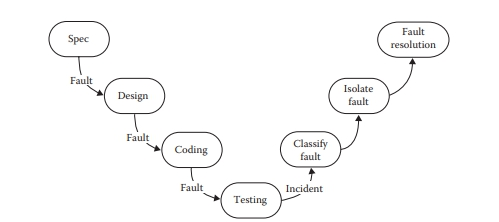
\includegraphics[scale=1.2]{gambar/cycle}
	\centering
	\caption{Siklus hidup pengujian.}
\end{figure}
Gambar 2.1 menggambarkan model siklus hidup untuk pengujian. Perhatikan bahwa, dalam fase pengembangan, tiga peluang muncul untuk membuat \textit{error}, yang menghasilkan \textit{fault} yang dapat menyebar melalui proses \textit{development}. Langkah resolusi \textit{fault} adalah kesempatan lain untuk \textit{error} (dan \textit{fault} baru). Ketika suatu perbaikan menyebabkan perangkat lunak yang sebelumnya benar untuk berperilaku salah, perbaikannya kurang[8].

Dari urutan \textit{term} ini, dapat dilihat bahwa \textit{test case} menempati posisi sentral dalam pengujian. Proses pengujian dapat dibagi lagi menjadi langkah-langkah terpisah: \textit{test planning, test case development}, menjalankan \textit{test case}, dan mengevaluasi hasil pengujian.Untuk \textit{test case} ada dua pendekatan mendasar digunakan untuk mengidentifikasi \textit{test case}; secara tradisional, ini disebut pengujian fungsional dan struktural. \textit{Specification-based} dan \textit{code-based} adalah nama yang lebih deskriptif. Kedua pendekatan memiliki beberapa metode identifikasi \textit{test case} yang berbeda; mereka umumnya hanya disebut metode pengujian.

\subsection{\textit{Specification-Based/Black-box Testing} [8]}
\paragraph{} 
Alasan bahwa pengujian berbasis spesifikasi pada awalnya disebut \textit{functional testing} adalah bahwa setiap program dapat dianggap sebagai fungsi yang memetakan nilai dari domain input ke nilai dalam rentang outputnya. Gagasan ini umumnya digunakan dalam \textit{engineering}, ketika suatu sistem dianggap sebagai \textit{black box}. Ini mengarah pada istilah sinonim lainnya — pengujian \textit{black-box}, di mana konten (implementasi) kotak hitam tidak diketahui, dan fungsi kotak hitam dipahami sepenuhnya dalam hal input dan outputnya (lihat Gambar 2.2). Sering kali, pengujian beroperasi sangat efektif dengan pengetahuan \textit{black box}; pada kenyataannya, ini adalah pusat orientasi objek. Sebagai contoh, kebanyakan orang berhasil mengoperasikan mobil dengan hanya pengetahuan "\textit{black box}".
\begin{figure}[h!]
	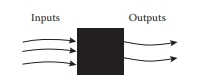
\includegraphics[scale=1.0]{gambar/blackbox}
	\centering
	\caption{Engineer’s black box.}
\end{figure}

Dengan pendekatan berbasis spesifikasi untuk menguji identifikasi kasus, satu-satunya informasi yang digunakan adalah spesifikasi perangkat lunak. Oleh karena itu, \textit{test case} memiliki dua keunggulan berbeda: 
\begin{enumerate}
\item Mereka tidak tergantung pada bagaimana perangkat lunak diimplementasikan, jadi jika implementasi berubah, \textit{test case} masih berguna.
\item Pengembangan \textit{test case} dapat terjadi secara paralel dengan implementasi, sehingga mengurangi keseluruhan interval pengembangan proyek.
\end{enumerate} 
Di sisi negatif, kasus uji berbasis spesifikasi sering mengalami dua masalah, redudansi yang signifikan mungkin ada di antara kasus uji, dan diperparah oleh kemungkinan kesenjangan perangkat lunak yang tidak diuji.

Gambar 2.3 menunjukkan hasil \textit{test case} yang diidentifikasi oleh dua metode berbasis spesifikasi. Metode A mengidentifikasi serangkaian kasus uji yang lebih besar daripada metode B. Perhatikan bahwa, untuk kedua metode, rangkaian kasus uji sepenuhnya terkandung dalam rangkaian perilaku tertentu. Karena metode berbasis spesifikasi didasarkan pada perilaku yang ditentukan, sulit untuk membayangkan metode ini mengidentifikasi perilaku yang tidak ditentukan.
\begin{figure}
	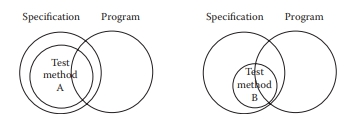
\includegraphics[scale=1.2]{gambar/compareAB}
	\centering
	\caption{Comparing specification-based test case identification methods}
\end{figure}
\subsection{\textit{Code-Based Testing/White-box Testing}}
\paragraph{}
Pengujian berbasis kode adalah pendekatan mendasar lainnya untuk menguji \textit{test case}. Untuk membandingkannya dengan pengujian \textit{black box}, kadang-kadang disebut pengujian \textit{white box} (atau bahkan \textit{clear box}). Metafora \textit{clear box} mungkin lebih tepat karena perbedaan mendasar adalah bahwa implementasi (\textit{black box}) diketahui dan digunakan untuk mengidentifikasi \textit{test case}. Kemampuan untuk "melihat ke dalam" \textit{black box} memungkinkan tester untuk mengidentifikasi \textit{test case} berdasarkan bagaimana fungsi tersebut benar-benar dijalankan.

Pengujian berbasis kode telah menjadi subjek dari beberapa teori yang cukup kuat. Dengan konsep-konsep ini, tester dapat dengan ketat menggambarkan dengan tepat apa yang akan diuji. Karena dasar teorinya yang kuat, pengujian berbasis kode cocok untuk menjadi definisi dan penggunaan \textit{test coverage metrics}. \textit{Test coverage metrics} menyediakan cara untuk secara eksplisit menyatakan sejauh mana \textit{item} perangkat lunak telah diuji, dan ini pada gilirannya membuat manajemen pengujian lebih jelas.

Gambar 2.4 menunjukkan hasil \textit{test case} yang diidentifikasi oleh dua metode berbasis kode. Seperti sebelumnya, metode A mengidentifikasi satu set kasus uji yang lebih besar daripada metode B. Apakah satu set kasus uji yang lebih besar tentu lebih baik? Ini adalah pertanyaan yang bagus, dan pengujian berbasis kode menyediakan cara-cara penting untuk mengembangkan jawaban. Perhatikan bahwa, untuk kedua metode, himpunan kasus uji sepenuhnya terkandung dalam himpunan perilaku yang diprogram. Karena metode berbasis kode didasarkan pada program, sulit membayangkan metode ini mengidentifikasi perilaku yang tidak diprogram. Sangat mudah untuk membayangkan, bagaimanapun, bahwa serangkaian kasus uji berbasis kode relatif kecil sehubungan dengan perilaku lengkap yang diprogram. 
\begin{figure}
 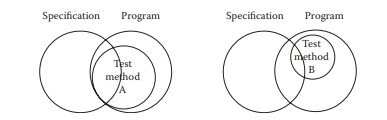
\includegraphics[scale=1.2]{gambar/compareAB-whitebox}
 \centering
 \caption{Comparing code-based test case identification methods.}
\end{figure}

\section{Bahasa Pemrograman PHP}
\label{php}

\section{Bahasa Pemrograman HTML}
\label{html}

\section{Codeigniter}
\label{ci}

\section{Code Coverage}
\label{codecoverage}

\section{Xampp}
\label{xampp}

\section{Travis CI}
\label{travis}


